\documentclass[handout]{beamer}
\usepackage[orientation=portrait,size=A4]{beamerposter} 

\usepackage[utf8]{inputenc}
\usepackage[T1]{fontenc}
\usepackage{fontspec}
\usepackage[french]{babel}
\usepackage{graphicx}
\usepackage{array}
\usepackage{pifont}
\usepackage{amsmath, amssymb}
\usepackage{wrapfig}
\usepackage{mwe}
\usepackage{tikz}
\usetikzlibrary{calc}
\usepackage{pgfplots}
\pgfplotsset{compat=1.3}
%\usepackage{pstricks,pst-plot,pstricks-add}

\newcommand{\tick}{\ding{52}}
\newcommand{\lnon}{\overline}

\graphicspath{{./images/}}


\newcommand{\ensemble}[1]{\left\lbrace{} #1 \right\rbrace{}}


%\usetheme{Boadilla}

\title{Optimisation de circuits logiques}
\author{Alexandre JANNIAUX}
\date{}

\begin{document}

\begin{frame}
  \maketitle
  \tableofcontents
\end{frame}

\section{Circuits logiques et fonctions combinatoires}
\begin{frame}
  \frametitle{Circuits logiques et fonctions combinatoires}
  %\begin{figure}[p]
  %  \includegraphics[width=8cm]{circuit_logique_pla.png}
  %  \caption{Exemple de circuit logique PLA ET/OU}
  %  \label{fig:circ1}
  %\end{figure}
  
  \[ \begin{aligned}
    f: \ensemble{0,1}^3 &\longrightarrow && \ensemble{0,1,\_} \\
    (e_1,e_2,e_3) & \longmapsto && (e_1+e_2)e_3 + (e_1+e_3)e_2
  \end{aligned}
  \]

  \textbf{Notations : }
  \begin{itemize}
  \item Mintermes : $A\lnon{B}C\lnon{D}EF = (1,0,1,0,1,1) = \overline{101011}^{2} = 43$
  \item DNF : $a_i$ : $f = \sum m(a_1, \cdots, a_n)$
  \item Terme simplifié : $(1,\_,0) = A\overline{C} = A(B+\overline{B})\overline{C}$
  %\item ON-set : $\mathcal{O} = f^{-1}(\{1\}) = \ensemble{(x_1,\cdots, x_n) \mid f=1}$
  %\item DC-set : $\mathcal{D} = f^{-1}(\{\_\})$ ``Don't care''
  \end{itemize}
  

  \begin{tikzpicture}[scale=2](3,3)
      \coordinate (A) at (0,2,2);
      \coordinate (B) at (2,2,2);
      \coordinate (C) at (2,0,2);
      \coordinate (D) at (0,0,2);
      \coordinate (E) at (0,0,0);
      \coordinate (F) at (0,2,0);
      \coordinate (G) at (2,2,0);
      \coordinate (H) at (2,0,0);
      
  	  \draw[thick](2,2,0)--(0,2,0)--(0,2,2)--(2,2,2)--(2,2,0)--(2,0,0)--(2,0,2)--(0,0,2)--(0,2,2);
  	  \draw[thick](2,2,2)--(2,0,2);
  	  \draw[gray](2,0,0)--(0,0,0)--(0,2,0);
 	  \draw[gray](0,0,0)--(0,0,2);
 	  
  	  \fill(A) circle (0.15);
  	  \fill(B) circle (0.15);
  	  \draw(C) circle (0.15);
  	  \draw(D) circle (0.15);
  	  \draw(E) circle (0.15);
  	  \draw(F) circle (0.15);
  	  \draw(G) circle (0.15);
  	  \draw(H) circle (0.15);
  	  
  	  
	  \coordinate (AB) at ($ (A)!.5!(B) $); 
  	  \draw (AB) ellipse (1.3 and 0.5);
  	  
  	  %\draw(1,1,2) node{1};
 	  %\draw(1,2,1) node{2};
 	  %\draw(2,1,1) node{3};
 	  %\draw[gray!20](1,0,1) node{4};
 	  %\draw[gray!20](0,1,1) node{5};
 	  %\draw[gray!20](1,1,0) node{6};
      \end{tikzpicture}
      
      
      % PERFORMANCES : 
      \begin{tikzpicture}[scale=1]
		\draw plot coordinates {(0,0) (1,0) (2,2) (3,0)
		(4,6) (5,4) (6,7) (7,4) (8,3) (9,0) (10,1)};
	  \end{tikzpicture}
% \begin{figure}[p]
%    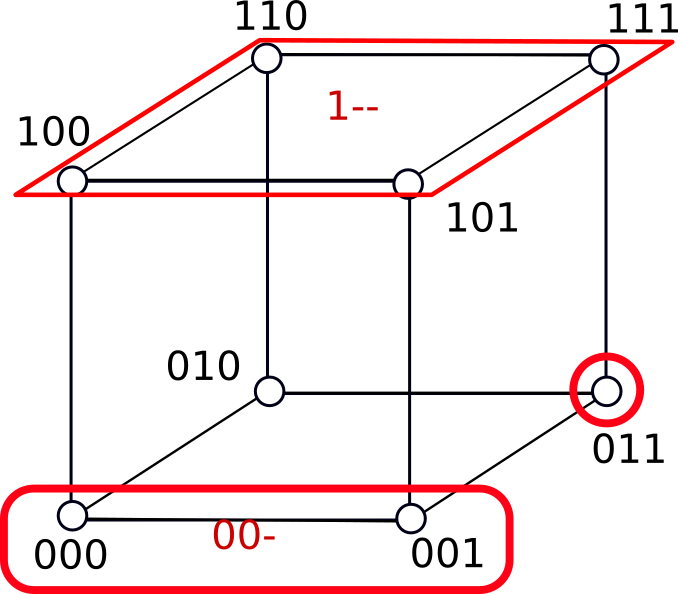
\includegraphics[width=8cm]{cube_qm.png}
%    \caption{Repr\'esentation graphique de minterme}
%    \label{fig:cube1}
% \end{figure}
  
  
  %\begin{figure}[p]
  % \input{'graph_rec.tex'}
  %\end{figure}
  

  
\end{frame}

\section{M\'ethode de Quine-McCluskey}
\begin{frame}
  \frametitle{M\'ethode de Quine-McCluskey}
  
  \textbf{Expansion des cubes :}
  
     \begin{tikzpicture}[scale=2]
     (9,3)
      \coordinate (A) at (0,2,2);
      \coordinate (B) at (2,2,2);
      \coordinate (C) at (2,0,2);
      \coordinate (D) at (0,0,2);
      \coordinate (E) at (0,0,0);
      \coordinate (F) at (0,2,0);
      \coordinate (G) at (2,2,0);
      \coordinate (H) at (2,0,0);
      
      \coordinate (A2) at (6,2,2);
      \coordinate (B2) at (8,2,2);
      \coordinate (C2) at (8,0,2);
      \coordinate (D2) at (6,0,2);
      \coordinate (E2) at (6,0,0);
      \coordinate (F2) at (6,2,0);
      \coordinate (G2) at (8,2,0);
      \coordinate (H2) at (8,0,0);
      
      % ARETES DROITE
      \coordinate (BC2) at ($ (B2)!.5!(C2) $);
      \coordinate (CD2) at ($ (C2)!.5!(D2) $); 
      \coordinate (FG2) at ($ (F2)!.5!(G2) $); 
      \coordinate (BG2) at ($ (B2)!.5!(G2) $);
      \coordinate (DE2) at ($ (D2)!.5!(E2) $);
      \coordinate (EF2) at ($ (E2)!.5!(F2) $);      
      
      % ARMATURE CUBE GAUCHE
  	  \draw[thick](G)--(F)--(A)--(B)--(G)--(H)--(C)--(D)--(A);
  	  \draw[thick](B)--(C);
  	  \draw[gray](H)--(E)--(F);
 	  \draw[gray](E)--(D);
 	  
 	  % ARMATURE CUBE DROIT
 	  \draw[thick](G2)--(F2)--(A2)--(B2)--(G2)--(H2)--(C2)--(D2)--(A2);
  	  \draw[thick](B2)--(C2);
  	  \draw[gray](H2)--(E2)--(F2);
 	  \draw[gray](E2)--(D2);
 	  
	  % FLECHE
	  \draw[ultra thick](4,1.4,2)--(5,1.4,2)--(5,1.6,2)--(5.5,1.2,2)--(5,0.8,2)--(5,1,2)--(4,1,2);
	  
	  % ELLIPSES GAUCHE
	  \draw[ultra thick] (BC2) ellipse (0.3 and 1.3); % Verticales
  	  \draw[ultra thick] (EF2) ellipse (0.3 and 1.3); 
	  \draw[ultra thick] (CD2) ellipse (1.3 and 0.3); % Horizontales
	  \draw[ultra thick] (FG2) ellipse (1.3 and 0.3); 
	  \draw[ultra thick, rotate around={45:(BG2)}] (BG2)  ellipse (1 and 0.3); % Oblique 
      \draw[ultra thick, rotate around={45:(DE2)}] (DE2)  ellipse (1 and 0.3); % Oblique 		  	  
	  	  
	  % ELLIPSES DROIT
	   	  
 	  
 	  % POINTS CUBE GAUCHE
  	  \draw(A) circle (0.15) node[below left] {$A$};
  	  \filldraw(B) circle (0.15) node[below right] {$B$};
  	  \filldraw(C) circle (0.15) node[below right] {$C$};
  	  \filldraw(D) circle (0.15) node[below left] {$D$};
  	  \filldraw(E) circle (0.15) node[below right] {$E$};
  	  \filldraw(F) circle (0.15) node[above left] {$F$};
  	  \filldraw(G) circle (0.15) node[above right] {$G$};
  	  \draw(H) circle (0.15) node[below right] {$H$};
  	  
  	  % POINTS CUBE DROIT
  	  \draw(A2) circle (0.15);
  	  \filldraw(B2) circle (0.15);
  	  \filldraw(C2) circle (0.15);
  	  \filldraw(D2) circle (0.15);
  	  \filldraw(E2) circle (0.15);
  	  \filldraw(F2) circle (0.15);
  	  \filldraw(G2) circle (0.15);
  	  \draw(H2) circle (0.15);
     \end{tikzpicture}

  \textbf{Performances :}     
     
     \begin{columns}
     	\begin{column}[t]{0.5\hsize}
	     \begin{tikzpicture}[scale=0.8]
    	 \begin{axis}[
	ymode=log,
	extra tick style={grid=major},
	title=Circuit premier,
	xlabel={nombre de variables},
	ylabel={temps ($s$)}]

\addplot table {images/expand_bench.dat};
	
\end{axis}
	
%\draw plot coordinates {
%(0,0) 
%(1,0) 
%(2,0) 
%(3,0)
%(4,0.003) 
%(5,0.014) 
%(6,0.07) 
%(7,0.33) 
%(8,1.8) 
%(9,10.8) %};
%(10,56.6)};
	     \end{tikzpicture}
	     \end{column}

     
	     \begin{column}[t]{0.5\hsize}
	     \begin{tikzpicture}[scale=0.8]
    	 \begin{axis}[
	xmode=log,
	ymode=log,
	extra tick style={grid=major},
	title=Circuit premier,
	xlabel={nombre de cubes},
	ylabel={temps ($s$)}]

\addplot table {images/expand_bench_cube.dat};
	
\end{axis}
	
%\draw plot coordinates {
%(0,0) 
%(1,0) 
%(2,0) 
%(3,0)
%(4,0.003) 
%(5,0.014) 
%(6,0.07) 
%(7,0.33) 
%(8,1.8) 
%(9,10.8) %};
%(10,56.6)};
	     \end{tikzpicture}
    	 \end{column} 
	  \end{columns}
%  \large{\textbf{Exemple :}} \[ f(x_1,\cdots,x_6) = \sum m(36, 44, 51, 60) \]
%
%  
%  \begin{minipage}[b]{0.5\hsize}\centering
%    \begin{tabular}{rl}
%      36: & 100100  \tick \\ \hline 
%      44: & 101100  \tick \\ 
%      51: & 110011   \\ \hline
%      60: & 111100 \tick
%    \end{tabular}
%  \end{minipage}
%  %
%  \begin{minipage}{0.4\hsize}\centering
%    \begin{tabular}{rl}
%      36,44: & 10\_100  \\ \hline 
%      44,60: & 1\_1100    
%    \end{tabular}
%  \end{minipage}
  
  %\large{\textbf{Idée :}} Une fonction combinatoire est définie par le langage accepté (couverture).
  
  %=> On utilise l'algèbre de Boole pour simplifier les expressions
  
  %\large{\textbf{Algorithme :}}
  %\begin{enumerate}
  %   \item 
  %\end{enumerate}
\end{frame}

\section{Méthode de Quine-McCluskey}
\begin{frame}
  \frametitle{Méthode de Quine-McCluskey}
  
  \textbf{Suppression des redondances inutiles : }
  
  \begin{tikzpicture}[scale=2]
  (9,3)
      \coordinate (A) at (0,2,2);
      \coordinate (B) at (2,2,2);
      \coordinate (C) at (2,0,2);
      \coordinate (D) at (0,0,2);
      \coordinate (E) at (0,0,0);
      \coordinate (F) at (0,2,0);
      \coordinate (G) at (2,2,0);
      \coordinate (H) at (2,0,0);
      
      \coordinate (A2) at (6,2,2);
      \coordinate (B2) at (8,2,2);
      \coordinate (C2) at (8,0,2);
      \coordinate (D2) at (6,0,2);
      \coordinate (E2) at (6,0,0);
      \coordinate (F2) at (6,2,0);
      \coordinate (G2) at (8,2,0);
      \coordinate (H2) at (8,0,0);
      
      % ARETES GAUCHE
      \coordinate (BC) at ($ (B)!.5!(C) $);
      \coordinate (CD) at ($ (C)!.5!(D) $); 
      \coordinate (FG) at ($ (F)!.5!(G) $); 
      \coordinate (BG) at ($ (B)!.5!(G) $);
      \coordinate (DE) at ($ (D)!.5!(E) $);
      \coordinate (EF) at ($ (E)!.5!(F) $);      
      
      % ARETES DROITE
      \coordinate (BC2) at ($ (B2)!.5!(C2) $);
      \coordinate (CD2) at ($ (C2)!.5!(D2) $); 
      \coordinate (FG2) at ($ (F2)!.5!(G2) $); 
      \coordinate (BG2) at ($ (B2)!.5!(G2) $);
      \coordinate (DE2) at ($ (D2)!.5!(E2) $);
      \coordinate (EF2) at ($ (E2)!.5!(F2) $);      
      
      
      % ARMATURE CUBE GAUCHE
  	  \draw[thick](G)--(F)--(A)--(B)--(G)--(H)--(C)--(D)--(A);
  	  \draw[thick](B)--(C);
  	  \draw[gray](H)--(E)--(F);
 	  \draw[gray](E)--(D);
 	  
 	  % ARMATURE CUBE DROIT
 	  \draw[thick](G2)--(F2)--(A2)--(B2)--(G2)--(H2)--(C2)--(D2)--(A2);
  	  \draw[thick](B2)--(C2);
  	  \draw[gray](H2)--(E2)--(F2);
 	  \draw[gray](E2)--(D2);
 	  
	  % FLECHE
	  \draw[ultra thick](4,1.4,2)--(5,1.4,2)--(5,1.6,2)--(5.5,1.2,2)--(5,0.8,2)--(5,1,2)--(4,1,2);
	  
	
	  % ELLIPSES GAUCHE
	  \draw[ultra thick] (BC) ellipse (0.3 and 1.3); % Verticales
  	  \draw[ultra thick] (EF) ellipse (0.3 and 1.3); 
	  \draw[ultra thick] (CD) ellipse (1.3 and 0.3); % Horizontales
	  \draw[ultra thick] (FG) ellipse (1.3 and 0.3); 
	  \draw[ultra thick, rotate around={45:(BG)}] (BG)  ellipse (1 and 0.3); % Oblique 
      \draw[ultra thick, rotate around={45:(DE)}] (DE)  ellipse (1 and 0.3); % Oblique 		  
	  
	  
	  % ELLIPSES DROITE
	  %\draw[ultra thick] (BC2) ellipse (0.3 and 1.3); % Verticales
  	  \draw[ultra thick] (EF2) ellipse (0.3 and 1.3); 
	  \draw[ultra thick] (CD2) ellipse (1.3 and 0.3); % Horizontales
	  %\draw[ultra thick] (FG2) ellipse (1.3 and 0.3); 
	  \draw[ultra thick, rotate around={45:(BG2)}] (BG2)  ellipse (1 and 0.3); % Oblique 
      %\draw[ultra thick, rotate around={45:(DE2)}] (DE2)  ellipse (1 and 0.3); % Oblique 		  	  
	  	  
	  % ELLIPSES DROIT
	   	  
 	  
 	  % POINTS CUBE GAUCHE
  	  \draw(A) circle (0.15);
  	  \filldraw(B) circle (0.15);
  	  \filldraw(C) circle (0.15);
  	  \filldraw(D) circle (0.15);
  	  \filldraw(E) circle (0.15);
  	  \filldraw(F) circle (0.15);
  	  \filldraw(G) circle (0.15);
  	  \draw(H) circle (0.15);
  	  
  	  % POINTS CUBE DROIT
  	  \draw(A2) circle (0.15);
  	  \filldraw(B2) circle (0.15);
  	  \filldraw(C2) circle (0.15);
  	  \filldraw(D2) circle (0.15);
  	  \filldraw(E2) circle (0.15);
  	  \filldraw(F2) circle (0.15);
  	  \filldraw(G2) circle (0.15);
  	  \draw(H2) circle (0.15);
  \end{tikzpicture}  
  
  
%  
%  \begin{minipage}[c][6cm]{\hsize}\centering
%    \begin{tabular}{|l|c|c|c|c|}
%      \hline %
%      Implicants & 36 & 44 & 51 & 60  \\ \hline
%      51 &  &  & X &  \\ \hline
%      36,44 & X & X &  &    \\ \hline
%      44,60 &  & X &  & X \\ \hline
%    \end{tabular}
%    \newline
%    
%  \end{minipage}
%
%  \textbf{Méthode de Petrick :} exacte, exemple
%  \[ g \equiv (P_1+P_2)(P_1+P_4+P_4)\cdots(P_7+P_9) \]
%
%  \textbf{Approximation :}
%  \begin{itemize}
%  \item plus rapide
%  \item approximation en $H_n$
%  \item adapté à plusieurs itérations
%  \end{itemize}
\end{frame}

\section{Fonctions multivaluées}
\begin{frame}
  \frametitle{Fonctions multivaluées}

  \textbf{Définition :}
  \[ f: \mathcal{P}_1 \times \cdots \times \mathcal{P}_n \longrightarrow \mathbb{B}^m \]

  \textbf{Littéraux :} 
  \[X_i^{S_i} = %
  \begin{cases}
    1 \text{ si } X_i \in S_i \\
    0 \text{ sinon}
  \end{cases}
  \quad \text{où } X_i \in \mathcal{P}_i \text{ et } \mathcal{S}_i \subset \mathcal{P}_i \]

  \textbf{Décomposition de Shannon :}
  \[ \bigcup_{i=1}^n c_i = 1 \implies f \equiv \bigcup_{i=1}^{n} f\,|_{C_i} \cap c_i \]

\end{frame}

\begin{frame}
  \frametitle{Espresso}

  \[ \bigcup_{i=1}^n c_i = 1 \implies f \equiv \bigcup_{i=1}^{n} f\,|_{C_i} \cap c_i \]

  \textbf{Atout :} Optimisation récursive

  \textbf{Initialisation :}
  
  \begin{itemize}
  \item Simplification
  \item Élimination des redondances
  \item Recherche des impliquants essentiels
  \end{itemize}

  \textbf{Algorithme :}
  % Tant qu'on peut le faire : 
  \begin{itemize}
  \item Réduction d'un impliquant.
  \item Simplification
  \item Élimination des redondances
  \end{itemize}
  
\end{frame}

\begin{frame}
  \frametitle{Conclusion}

  \begin{itemize}
  \item Problème difficile...
  \item ...mais bien maîtrisé.
  \item Approximable facilement.
  \item Généralisable (XOR-NAND)

  \end{itemize}

\end{frame}

\end{document}
